% !TeX root = RJwrapper.tex


\title{\pkg{rotations}: A Package for $SO(3)$ Data}
\author{by Bryan Stanfill, Heike Hofmann, Ulrike Genschel}

\maketitle

%<<setup, include=FALSE, cache=FALSE>>=
%opts_chunk$set(fig.path='figures/', fig.align='center', fig.show='hold',comment=NA,background='white',highlight=FALSE,size='small')
%options(replace.assign=TRUE,width=90)
%library(rotations2)
%@

\abstract{
In this article we introduce the \pkg{rotations} package which provides users with the ability to simulate, analyze and visualize three-dimensional rotation data.  The \pkg{rotations} package includes four distributions from which to simulate data, four estimators of the central orientation and a novel approach to visualizing these data.  All of the above features are available to two different parameterizations of rotations: 3-by-3 matrix form and quaternions.
}

\section{Introduction}

Data in form of three-dimensional rotations find application in several scientific areas, such as bio-medical engineering, computer visioning, and geological and materials sciences.  A common goal shared by these fields is to estimate the main or central orientation for a sample of rotations.  That is, letting the rotation group $SO(3)$ denote the collection of all $3\times 3$ rotation matrices, observations $\bm{R}_1,\ldots,\bm{R}_n \in SO(3)$ can be conceptualized as a random sample from a \textit{location model}
\begin{equation}
\label{eqn:loc_model}
\mathbf{R}_i = \bm{S} \bm{E}_i, \quad i=1,\ldots,n,
\end{equation}
where $\bm S \in SO(3)$ is the {\it fixed} parameter of interest indicating an orientation of central tendency, and $\bm{E}_1,\ldots,\bm{E}_n \in SO(3)$ denote i.i.d. {\it random} rotations which symmetrically perturb $\bm{S}$.

The \pkg{rotations} package provides users with the tools necessary to simulate data from four common choices of symmetric distributions, estimate $\bm{S}$ in \eqref{eqn:loc_model} and visualize a sample of rotations.  The remainder of this paper is organized as follows.  We will begin with a discussion on how rotation data can be parameterized.  Then we discuss how data generation is possible in this package.  Next we discuss the different estimators used to estimate the central direction.  Finally, visualizations of rotation data is presented.

%For example, \citet{rancourt00} examine rotation matrix data in studying body positions whilst operating machinery. \cite{fletcher09} consider this type of  orientation data in magnetic resonance imaging and in shape analysis; similar examples  can be found in \cite{schwartz05}, \cite{pierrynowski09},  \cite{dai10},  or \cite{hadani11}.  The data in our illustrative example to follow arise from a study in materials science, where $3 \times 3$ rotations represent the orientations of cubic crystals on the micro-surface of a metal specimen as measured through electron backscatter diffraction (EBSD) and ``grains" within metals are composed of crystals which roughly share a common orientation; see \cite{randle03} for details on EBSD data.  
     
%From a sample of orientations, an important interest is often the estimation of a main or central orientation $\bm S$.  That is, letting the rotation group $SO(3)$ denote the collection of all $3\times 3$ rotation matrices, observations $\bm{R}_1,\ldots,\bm{R}_n \in SO(3)$ can be conceptualized as a random sample from a \textit{location model}
%\begin{equation}
%\label{eqn:1}
%\mathbf{R}_i = \bm{S} \bm{E}_i, \quad i=1,\ldots,n,
%\end{equation}
%where $\bm S \in SO(3)$ is the {\it fixed} parameter of interest indicating an orientation of central tendency, and $\bm{E}_1,\ldots,\bm{E}_n \in SO(3)$ denote iid {\it random} rotations which symmetrically perturb $\bm{S}$. The data-generating model in \eqref{eqn:1} is a rotation-matrix analog of a location model for scalar data $Y_i = \mu + e_i$, where $\mu \in \mathbb{R}$ denotes a mean and $e_i \in \mathbb{R}$ denotes an additive error symmetrically distributed around zero.  This representation \eqref{eqn:1} for orientations is quite common and, in fact, a variety of parametric models exist for describing symmetrically distributed rotations $\bm{E}_i$, such as the symmetric matrix Fisher distribution \citep{downs72}, the symmetric Cayley distribution \citep{leon06}  and the circular-von-Mises-based rotation distribution \citep{bingham09}   in the statistics literature, as well as the Bunge distribution \citep{bunge82}, the isotropic Gaussian distribution \citep{matthies88, savyolova95} and the de la Vall\'{e}e Poussin distribution \citep{Schaeben97} in the materials science literature. Our goal in the following is to summarize and compare the most frequently proposed approaches for point estimation of $\bm S$ based on sample \eqref{eqn:1} of orientation data.  Depending on the scientific literature, the approaches can be quite different.

%The topic of location estimation has received considerable attention for directional data on circles or spheres, \citep[see][]{fisher53, karcher77, khatri77, fisher85, ducharme87, bajaj88, liu92, chan93, mardia00}, but less is known about  estimator properties with rotation data.  As a compounding factor, several current approaches to estimating $\bm S$ have arisen out of literatures having differing statistical and geometrical emphases.  In the  applied sciences literature, estimators of $\bm S$ are typically based on distance measures involving {\it non-Euclidean} (i.e., Riemannian) geometry, such as the \emph{geometric mean} \citep{arun87, horn88, umeyama91, moakher02} or, more recently, the \emph{geometric median} \citep{fletcher08, fletcher09}.  Preferences may depend on outliers in the data, but such suggestions for estimating $\bm S$ often do {\it not} consider the potential impact of the underlying data-generating mechanism.   On the other hand, approaches in the statistical literature tend to motivate an estimator for $\bm S$  through likelihood or moment-estimation principles applied to a specifically assumed distributional model (e.g., matrix Fisher or Cayley distribution) for the symmetric rotation errors $\bm E_i$ \citep{downs72, jupp79, leon06, bingham10}. Almost always, this estimator turns out to be a \emph{projected arithmetic mean} based on {\it Euclidean} geometry. Hence, in addition to potential distributional assumptions, more fundamental divisions in estimation approaches may be attributable to different geometrical perspectives with rotation data.  

%Considering the potential effects of an underlying data generation model as well as the choice of geometry (i.e., Euclidean vs.~Riemannian), the above discussion indicates a need to investigate and identify good point estimators for rotation data.  In particular, because estimators in the applied sciences literatures  are often selected without decision-theoretical considerations based on underlying distributions, it is of interest to understand how different location estimators behave across common distributions for rotations.  In this paper, we evaluate four common estimators for $\bm S$ in the context of the location model \eqref{eqn:1}. These are either mean- or median-based, and either Euclidean- or Riemannian-based in geometry; the median- and Euclidean-based estimator is new here but its inclusion is natural and its performance can be generally quite good and (as will be evidenced) broadly recommendable.   Through simulation, we compare how these estimators perform with respect to three common probability models for symmetric rotation errors as defined in \eqref{eqn:1}, namely the circular-von Mises-based distribution, the symmetric matrix Fisher distribution and the symmetric Cayley distribution.  The matrix Fisher is arguably the most common distribution in the statistics literature \citep[see][]{chikuse03}. While not noted previously, the symmetric Cayley and the de la Vall\'{e}e Poussin distribution are in fact the same; the de la Vall\'{e}e Poussin distribution has been advocated in the material science literature \citep{Schaeben97}.   The circular-von Mises-based distribution is included because the distribution is non-regular and has been applied to EBSD data \citep{bingham09}.  We describe how error distribution structures for rotation data, in particular their variability and tail behavior, translate into performance differences among point estimators based on varying geometric considerations.

\section{Rotation Representations}

The variety of applications for rotations is echoed by the number of equivalent ways to parameterize them.  We consider three of the most popular: matrices in $SO(3)$ and unit quaternions.  

\subsection{Matrix Form}

Three-dimensional rotations can be represented by $3\times3$ orthogonal matrices with determinant one.  All matrices with these characteristics form a group called the {\it special orthogonal group}, or {\it rotation group}, denoted $SO(3)$.  Every element in $SO(3)$ can be described by an angle, $r\in[0,\pi)$ and an axis, $\bm u\in\mathbb{R}^3$ with $\|\bm u\|=1$. Thus $\bm{R}\in SO(3)$ can be thought of as rotating the coordinate axis, $\bm{I}_{3 \times 3}$, about the axis $\bm{u}$ by the angle $r$.  We adopt the material scientist's terminology in calling $r$ the misorientation angle and $\bm u$ the misorientation axis.

More specifically, given an angle, $r$, and axis, $\bm u$, a $3\times 3$ rotation matrix can be formed by
\begin{equation}\label{eqn:angleaxis}
 \bm{R} = \bm{R}(r,\bm{u}) = \bm{u}\bm{u}^\top+(\bm{I}_{3\times3}-\bm{u}\bm{u}^\top)\cos(r) +\Phi(\bm{u})\sin(r)
\end{equation}
where
\[
\Phi(\bm{u}) = \Phi (u_1,u_2,u_3) = \left(\begin{array}{ccc}0 & -u_3 & u_2 \\ u_3 & 0 & -u_1 \\-u_2 & u_1 & 0\end{array}\right).
\]

%The function \code{SO3} will form the rotation matrix corresponding to a given angle and axis of rotation.  One can also go the other direction with the functions \code{angle} and \code{axis}, which will return the angle and axis, respectively, for a given rotation matrix.  

% Next, \eqref{eqn:angleaxis} can be used with the following facts to find $\bm u$: $\bm{uu}^\top$ and $(\bm{I}_{3\times3}-\bm{u}\bm{u}^\top)$ are symmetric, $\Phi(\bm u)$ is skew-symmetric implying $\Phi(\bm u)^\top=-\Phi(\bm u)$.  Now form $\bm R-\bm R^\top$:
% \[
% \bm R-\bm R^\top=\Phi(\bm u)\sin(r)-\Phi(\bm u)^\top\sin(r)=2\sin(r)\Phi(\bm u).
% \]
% Now let $\bm V=2\sin(r)\Phi(\bm u)$ then by the definition of $\Phi(\cdot)$, $u_1=-\bm V_{2,3}/2\sin(r)$, $u_2=\bm V_{1,3}/2\sin(r)$ and $u_3=-\bm V_{1,2}/2\sin(r)$.  The function \code{axis} will perform this calculation.

\subsection{Quaternion Form}

A second parameterization of rotations is with a {\it quaternion} of unit length.  Quaternions are a form of imaginary numbers with one real entry and a vector of three imaginary parts that can be expressed as
\[
q = x_1 + x_2 i + x_3 j + x_4 k
\]
where $i,j,$ and $k$ are square roots of -1, i.e. $i^2 = j^2= k^2 = -1$.  We can write $q=(s,\bm v)$ as tuple of the scalar $s$ for coefficient {\bf 1} and vector $\bm v$ for the imaginary coefficients, i.e. $s=x_1$ and $\bm v= (x_2, x_3, x_4)$.

A rotation around axis $\bm u$ by angle $r$ translates to $q=(s,\bm v)$ with
\[
s = \cos{(r/2)},  \ \ \bm v = \bm u \sin {(r/2)}
\]
This makes $q$ a unit quaternion.  The following code forms a unit quaternion from an angle sampled uniformly from the interval $[-\pi,\pi]$ and an axis sampled uniformly from the unit circle.
%To form a quaternion given an angle and axis, use the function \code{Q4}.

%As with the matrix representation the \code{angle} and \code{axis} functions will extract an angle and axis from a quaternion.  One can use the functions to form a matrix from a quaternion, or simply use the function \code{SO3} with a \code{Q4} object as input.  Similarly, an object of class \code{SO3} can be made into a rotation matrix by using the \code{Q4} function.

%This form is popular with mathematicians and others interested in the theory of rotations because their form makes them simple to deal with in certain situations.

% \subsection{Euler Angle Form}
% 
% The final parameterization we consider is {\it Euler angles}.  Euler angles are three dimensional vectors describing a sequence of rotations of some fixed coordinate axis.  There are several versions of Euler angles and we consider the $z-x-z$ formulation.  That is, the orintation $\bm R\in SO(3)$ can be represented as $\bm e=(\alpha,\beta,\gamma)$  where $\alpha,2\beta,\gamma\in[0,2\pi]$.  This specific formulation of $\bm e$ can form a rotation by rotating the identity about the $z$-axis counterclockwise through $\alpha$ radians, then rotate the $x$-axis through $\beta$ radians and finally rotate the $z$-axis through $\gamma$ radians.
% 
% To make this more concrete, we can form the rotation matrix, $\bm R\in SO(3)$ from a vector of Euler angles, $(\alpha,\beta,\gamma)$, as follows.  Let $\bm e_1=\begin{bmatrix} 1&0&0\end{bmatrix}$ and $\bm e_3=\begin{bmatrix} 0&0&1\end{bmatrix}$ then using the notation from \eqref{eqn:angleaxis},
% \[
% \bm R=\bm R(\gamma,\bm e_1)\bm R(\beta,\bm e_3)\bm R(\alpha,\bm e_1).
% \]
% 
% For each of these parameterizations we have created a class of R objects: \code{SO3} for the matrix representation, \code{Q4} for quaternions and \code{EA} for Euler angles.  The names of these classes  are also functions that will return an object of the class with the same name given an angle and axis, or an object of any other class.  See the below code for an illustration.  First I generate a rotation matrix from an angle, $r$, and an axis, $\bm U$ using the function \code{SO3}.  Next we transform that rotation into quaternions then Euler angles with the funcions \code{Q4} and \code{EA}, respecitvely.  One can also create quaternions or Euler angles directly by feeding the angle and axis into those same functions.

%<<params>>=
%r<-runif(1,-pi,pi)
%theta<-acos(runif(1, -1, 1))
%phi<-runif(1, -pi, pi)
%U<-c(sin(theta)*cos(phi),
%		 sin(theta)*sin(phi),cos(theta))
%R<-SO3(U,r)
%q<-Q4(R)
%@
%As before the function \code{axis} and \code{angle} will extract the axis and angle of the Euler angle.  One can also translate an Euler angle into a quaternion or matrix by passing an \code{EA} object into \code{Q4} and \code{SO3}, respectively.  One can go the other direction too.

For the remainder of this article we will present our work using the matrix representation.  All the functions to follow will work with any of  the representations we have discussed above.

\section{Data generation} 

From \eqref{eqn:loc_model}, one can simulate a matrix $\bm{R}_i\in SO(3)$ by picking an axis $\bm u$ uniformly on the sphere then drawing an angle $r$ from a distribution symmetric about $0$ and bounded between $-\pi$ and $\pi$ then applying \eqref{eqn:angleaxis}.  A matrix generated in this fashion is said to belong to the \dfn{uniform-axis random spin}, or UARS, class of distributions and has the density
\begin{equation}\label{eq:uarsden}
f(\bm E_i|\kappa)=\frac{4\pi}{3-\tr(\bm E_i)}C\left(\left.\cos^{-1}\left\{\frac{1}{2}[\tr(\bm E_i)-1]\right\}\right|\kappa\right)
\end{equation}
where $C(\cdot|\kappa)$ is distribution function connecting to the angle of rotation $r$ \citep{bingham2009}.  Members of the UARS family of distributions are distinguished based on the angluar distribution.


The \pkg{rotate} package allows the user access to four members of the UARS class.  Each member is differentiated by the distribution function for $r$: the uniform distribution on the circle, the matrix Fisher \citep{langevin2005, downs1972, khatri1977, jupp1979}, the Cayley  \citep{Schaeben1997, leon2006} and a circular-von Mises-based distribution \citep{bingham2009}. 

%A general construction approach exists for random rotations that are symmetrically distributed around the identity matrix $\bm{I}_{3 \times 3}$; see \citet{watson83, bingham09} and \citet{hielscher10}.  To this end, let $\bm{U}\in\mathbb{R}^3$ represent a point chosen uniformly on the unit sphere and, independently, generate a random angle $r$ according to some circular density $C(r|\kappa)$ on $(-\pi,\pi]$, which is symmetric around 0 and where $\kappa$ denotes a concentration parameter governing the spread of the circular distribution.  Then, define a random rotation as $\bm{E}=\bm{E}(\bm{U},r)$ using the constructive definition \eqref{eqn:angleaxis} (i.e., $\bm{E}$ represents the position of $\bm{I}_{3\times 3}$ upon rotating the standard coordinate frame in $\mathbb{R}^3$ about the random axis $\bm{U}$ by the random angle $r$).  The resulting rotation $\bm{E}$ will be symmetrically distributed and its distributional type (i.e., matrix Fisher, Cayley or circular-von Mises-based) is determined by the form of the circular density $C(r|\kappa)$ for the (misorientation) angle $r$.

The uniform distribution on the circle is given by the following density function
\begin{equation}\label{eqn:haar}
C_\mathrm{{H}}(r)=\frac{1-\cos(r)}{2\pi}
\end{equation}
for $r\in(-\pi,\pi]$.  This function also plays the part of a measure on the sphere, called the Haar measure on the sphere.  The function \code{rhaar} with input \code{n} will draw a sample of size $n$ from \eqref{eqn:haar} and \code{dhaar} with evaluate the density at a given point.

The following three distributions are all symmetric around $0$ on the range $[-\pi,\pi)$ and have one parameter, $\kappa$, which is the concentration parameter.  As $\kappa$ increases, the distribution becomes more peaked about $0$ and less variable.  If one would prefer to specify the variability instead, the circular variance denoted $\nu$ can also be set by the user.  For $r\sim F$ where $F$ is a distribution on the circle, the circular variance is defined as $\nu=1-E\cos(r)$, and $E\cos(r)$ is called the mean resultant length \citep{mardia2000}.

The symmetric matrix Fisher distribution is the oldest and also the most difficult to sample from.  It takes on the following distributional form
\[
C_\mathrm{{F}}(r| 
\kappa)=\frac{1}{2\pi[\mathrm{I_0}(2\kappa)-\mathrm{I_1}(2\kappa)]}e^{2\kappa\cos(r)}[1-\cos(r)]
\]
where $\mathrm{I_p}(\cdot)$ denotes the Bessel function of order $p$ defined as  $\mathrm{I_p}(\kappa)=\frac{1}{2\pi}\int_{-\pi}^{\pi}\cos(pr)e^{\kappa\cos r}dr$.  

For a given $\kappa$, the function \code{rfisher} generates a sample of size $n$ from this distribution using a rejection algorithm and \code{dfisher} evaluates the density at a given angle $r$.

\citet{leon2006} proposed the symmetric Cayley distribution, which is identical to the de la Vall\'{e}e Poussin distribution and a favorite among material scientists \citep{Schaeben1997}.  This distribution is closely related to the beta distribution and has the distributional form
\[
C_\mathrm{C}(r |\kappa)=\frac{1}{\sqrt{\pi}} \frac{\Gamma(\kappa+2)}{\Gamma(\kappa+1/2)}2^{-(\kappa+1)}(1+\cos r)^\kappa(1-\cos r).
\]
\code{rcayley} simulates from this distribution by taking a simple transformation of random deviates from a beta distribution and \code{dcayley} evaluates the Cayley density at a given angle, $r$.

Finally the circular-von Mises-based distribution is included because the distribution is non-regular and has been applied to EBSD data \citep{bingham2009}.  An angle following this distribution has the distribution form
\[
C_\mathrm{M}(r|\kappa)=\frac{1}{2\pi \mathrm{I_0}(\kappa)}e^{\kappa\cos(r)}.
\]
Simulation from this distribution was developed by \citet{best1979} and the function \code{rvmises} follows this procedure closely.  Also, \code{dvmises} evaluates the density at a given angle, $r$.

Once an angular distribution has been chosen and a vector of $n$ angles of rotation have been generated, the \code{genR} function with argument \code{space="SO3"} creates an $n\times 9$ matrix representing a sample from the appropriate UARS member as demonstrated in the following code.  If quaternions are required the argument \code{space} can be changed to \code{"Q4"}.

%<<genRs>>=
%Rs<-ruars(20,rcayley,kappa=1)
%matrix(Rs[1,],3,3)
%@

Here \code{rcayley(20,1)} simulates $r_1,\ldots,r_{20}$ from  $C_\mathrm{C}(r |\kappa=1)$ then \code{genR} generates the matrices.  Each row of \code{Rs} is an element in $SO(3)$, as demonstrated by \code{is.SO3}, in vector form with central orientation $\bm I_{3\times 3}$.  Any other central orientation in $SO(3)$ is possible by changing the \code{S} argument.  If a central orientation not in $SO(3)$ is proposed, however, an error is returned.

\section{$SO(3)$ data analysis\label{section:analysis}}

Given a sample of $n$ observations $\bm R_1,\dots,\bm R_{n}$ generated according to \eqref{eqn:loc_model} we offer four ways to estimate the central orientation $\bm S$.  These estimators are either Riemannian- or Euclidean-based in geometry and either mean- or median-based.  First we discuss how the choice of geometry affects distance.

The choice of geometry results in two different metrics to measure the distance between rotation matrices $\bm{R}_1$ and $\bm{R}_2 \in SO(3)$. Under the embedding approach, the natural distance metric between two random matrices in the Euclidean distance, $\Edist$, is induced by the Frobenius norm 
\begin{equation}
\label{d_E}
\Edist(\bm{R}_1,\bm{R}_2)=\|\bm{R}_1-\bm{R}_2\|_F, 
\end{equation}
where $\|\bm{A}\|_F = \sqrt{\mathbf{tr}({\bm A^\top \bm A})}$ denotes the Frobenius norm of a matrix $\bm A$ and $\mathbf{tr}(\cdot)$ denotes the trace of a matrix.  The Euclidean distance between two rotation matrices corresponds to the shortest cord in $\mathcal{M}(3)$ that connects them.  If $r\in[-\pi,\pi)$ denotes the misorientation angle in the angle-axis representation \eqref{eqn:angleaxis} of $\bm{R}_1^\top \bm{R}_2 \equiv \bm{R}_1^\top \bm{R}_2(r,\bm{u})$ (so that $\mathbf{tr}(\bm{R}_1^\top \bm{R}_2) =1 +2 \cos r$), then $\Edist(\bm{R}_1,\bm{R}_2) = 2\sqrt{2}\sin(|r|/2)$ holds.

By staying in the Riemannian space $SO(3)$ under the intrinsic approach, the natural distance metric becomes the Riemannian (or geodesic) distance, $\Rdist$, by which the distance between two rotations $\bm{R}_1,\bm{R}_2\in SO(3)$  is  defined as 
\begin{equation}
\label{d_R}
\Rdist(\bm{R}_1,\bm{R}_2)=  \frac{1}{\sqrt{2}}\|\text{Log}(\bm{R}_1^\top\bm{R}_2)\|_F = |r|,
\end{equation}
where $\text{Log}(\bm{R})$ denotes the principle logarithm of $\bm{R}$ (i.e., $\text{Log}(\bm{R}) = \text{Log}(\bm{R}(\bm u,r))= \bm \Phi(r\bm u)$ in \eqref{eqn:angleaxis}) and $r\in[-\pi,\pi)$ is the misorientation angle of $\bm{R}_1^\top \bm{R}_2$.  The Riemannian distance corresponds to the length of the shortest path that connects $\bm{R}_1$ and $\bm{R}_2$ {\it within} the space $SO(3)$. For this reason, the Riemannian distance is often considered the more natural metric on $SO(3)$; see \citet{moakher2002} for this discussion along with more details on exponential/logarithmic operators related to $SO(3)$.

We first consider estimators based on the embedding approach, which we call the projected estimators.  The median-based estimator in this class is
\begin{equation}\label{est:med}
\ProjMedian=\argmin_{\bm{S}\in
SO(3)}\sum_{i=1}^n\Edist(\bm{R}_i,\bm{S}).
\end{equation}
The function \code{median} with argument \code{type="projected"} approximates $\ProjMedian$ and uses an adaptation of the Weiszfeld algorithm \citep{weiszfeld1937}.  The mean-based estimator is 
\begin{align}\label{est:pam}
\ProjMean&=\argmin_{\bm{S}\in
SO(3)}\sum_{i=1}^n\Edist^2(\bm{R}_i,\bm{S})\nonumber\\
&=\argmax_{\bm{S}\in
SO(3)}\tr(\bm{S}^{\top}\overline{\bm{R}})
\end{align}
and is computed by the function \code{mean} with argument \code{type="projected"}.  For an in-depth discussion of the algorithm used to compute this value consult \citet{moakher2002}.

The geometric estimators minimize the first and second order Riemannian distances.  The \dfn{geometric median} is 
\begin{equation}\label{est:lone}
\GeoMedian=\argmin_{\bm{S}\in
SO(3)}\sum_{i=1}^n\Rdist(\bm{R}_i,\bm{S}).
\end{equation}
An algorithm proposed by \citet{hartley2011} is employed by the function \code{median} with argument \code{type="geometric"}.  The \dfn{geometric mean} is the $L_2$ analog of $\GeoMedian$ given by 
\begin{equation}\label{est:ltwo}
\GeoMean=\argmin_{\bm{S}\in
SO(3)}\sum_{i=1}^n\Rdist^2(\bm{R}_i,\bm{S}).
\end{equation}
The function \code{mean} with argument \code{type="geometric"} implements an algorithm first proposed by \citet{manton2004} in estimating $\GeoMean$.

\section{Confidence Regions}

Asymptotic results for the projected mean $\ProjMean$ can be used to infer about the central orientation $\bm S$. In particular, results in \cite{prentice1986,chang2001} and Zhang et al. (2009) give three distinct approaches to forming a confidence region for the central orientation.  The \code{region} function acts as a wrapper that can be used to access each of these methods for a sample from \eqref{eqn:loc_model} through the \code{method} argument.


The first method we consider is due to \cite{prentice1986} and is based upon asymptotic results for eigenvectors.  \cite{rancourt2000} used this method in the context of human kinematics and we use their formulation of the result.  A call to the \code{region} function with argument \code{method="prentice"} will return a vector of length three, where each value corresponds to the largest possible radius of the confidence region centered at each axis of $\ProjMean$.  A conservative estimate of the overall confidence region is therefore the largest of the three returned values.

The second method we consider is based upon a result given by \cite{chang2001} that was later clarified for the UARS context by Stanfill et al. (2013).  For this case, the \code{region} function with \code{method="chang"} returns a single value that represents the largest radius possible for the confidence region centered at $\ProjMean$.

The final method available is due to Zhange and Nordman (2009) and is a non-parametric pivotal bootstrap method.  When \code{method="zhang"} is specified the additional \code{m} argument specifices how large a bootstrap sample size to use in order to estimate the critical value, which is used in place of the $\chi^2_3$ percentile.  The simulation study in Stanfill et al. (2013) indicates that this is the best region estimation procedure in terms of coverage rate, especially for small sample sizes.


% \section{Confidence Area Construction}
% 
% With limited theory available for estimators of the central orientation, a bootstrap method is proposed to estimate the uncertainty associated with them.  The procedure implemented by the function \code{CIradius} is as follows where $\widehat{\bm S}$ is any of the estimators discussed so far:
% \begin{enumerate}
% \item Estimate $\widehat{\bm S}$ from $(\bm R_1,\dots,\bm R_n)$ 
% \item Sample $\bm R_1$,...,$\bm R_m$ from $(\bm R_1,\dots,\bm R_n)$ with replacement
% \item Estimate $\widehat{\bm S}^*$ from bootstrap sample
% \item Compute $\hat{T}=d_G(\widehat{\bm S},\widehat{\bm S}^*)$
% \item Repeat steps 1-3 B times
% \item Report q\% percentile of $\hat{T}$ to be the radius of the confidence `cone'
% \end{enumerate}
% A similar procedure was used by \cite{bingham10}, but in place of $\Rdist$ the maximum absolute angle between all three axis, which they called $\alpha$, was used.  It's easy to show that $\alpha$ is less than or equal to the geodesic distance between any two rotations making our method slightly more conservative.

\section{Visualizations}
In this section we introduce a method to visualize $SO(3)$ data via the the \pkg{ggplot2} package \citep{wickham2009}.  The function \code{plot} takes as input a $n\times 9$ matrix of $SO(3)$ observations and returns a visualization of one of the three columns.  The user can specify which column to use with the \code{col} argument, the default is one.  If the data are highly concentrated in one part of the sphere then the the \code{to$\_$range} argument can be set to \code{TRUE} then the range of the plot is set to zoom in on the populated area. 

Any of the four estimates of the central direction can be plotted along with a sample of rotations. To show all estimates at once add the argument \code{estimates$\_$show="all"}.  If only a few estimates are of interest then any combination of \code{"proj.mean"}, \code{"proj.median"}, \code{"riem.mean"} or \code{"riem.median"} are valid inputs.  The estimators are indicated by shape.  One can also center the data about any observation in $SO(3)$ by setting \code{center=S}.   Typically take \code{center=mean(Rs)}.  

\begin{example}
Rs<-ruars(50,rcayley,kappa=1)
plot(Rs,center=id.SO3)
plot(Rs,center=id.SO3,show_estimates='all')
plot(Rs,center=id.SO3,show_estimates='proj.mean',
		 show_regions='all',alp=.1)
\end{example}

%<<eye,fig.width=6,fig.height=6,echo=FALSE,include=FALSE>>=
%Rs<-ruars(50,rcayley,kappa=1)
%plot(Rs,center=id.SO3)
%plot(Rs,center=id.SO3,show_estimates='all')
%plot(Rs,center=id.SO3,show_estimates='proj.mean',
%		 show_regions='all',alp=.1)
%@


\begin{figure}
\centering
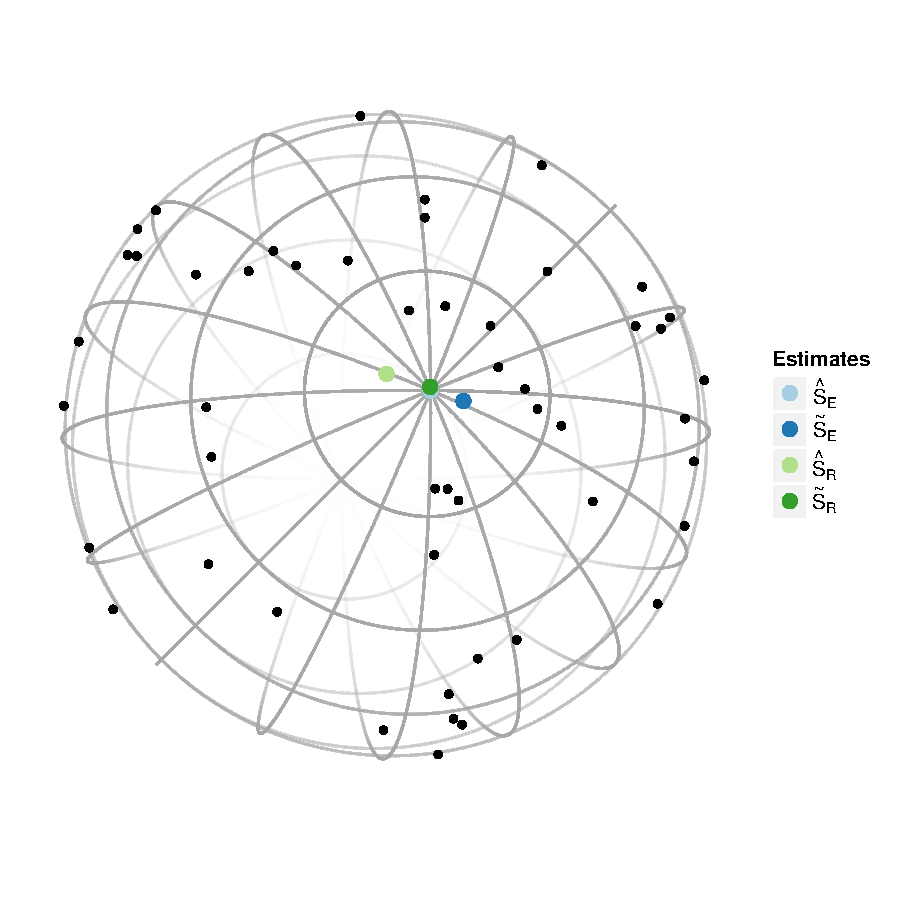
\includegraphics[width=.6\textwidth]{figures/eye}
%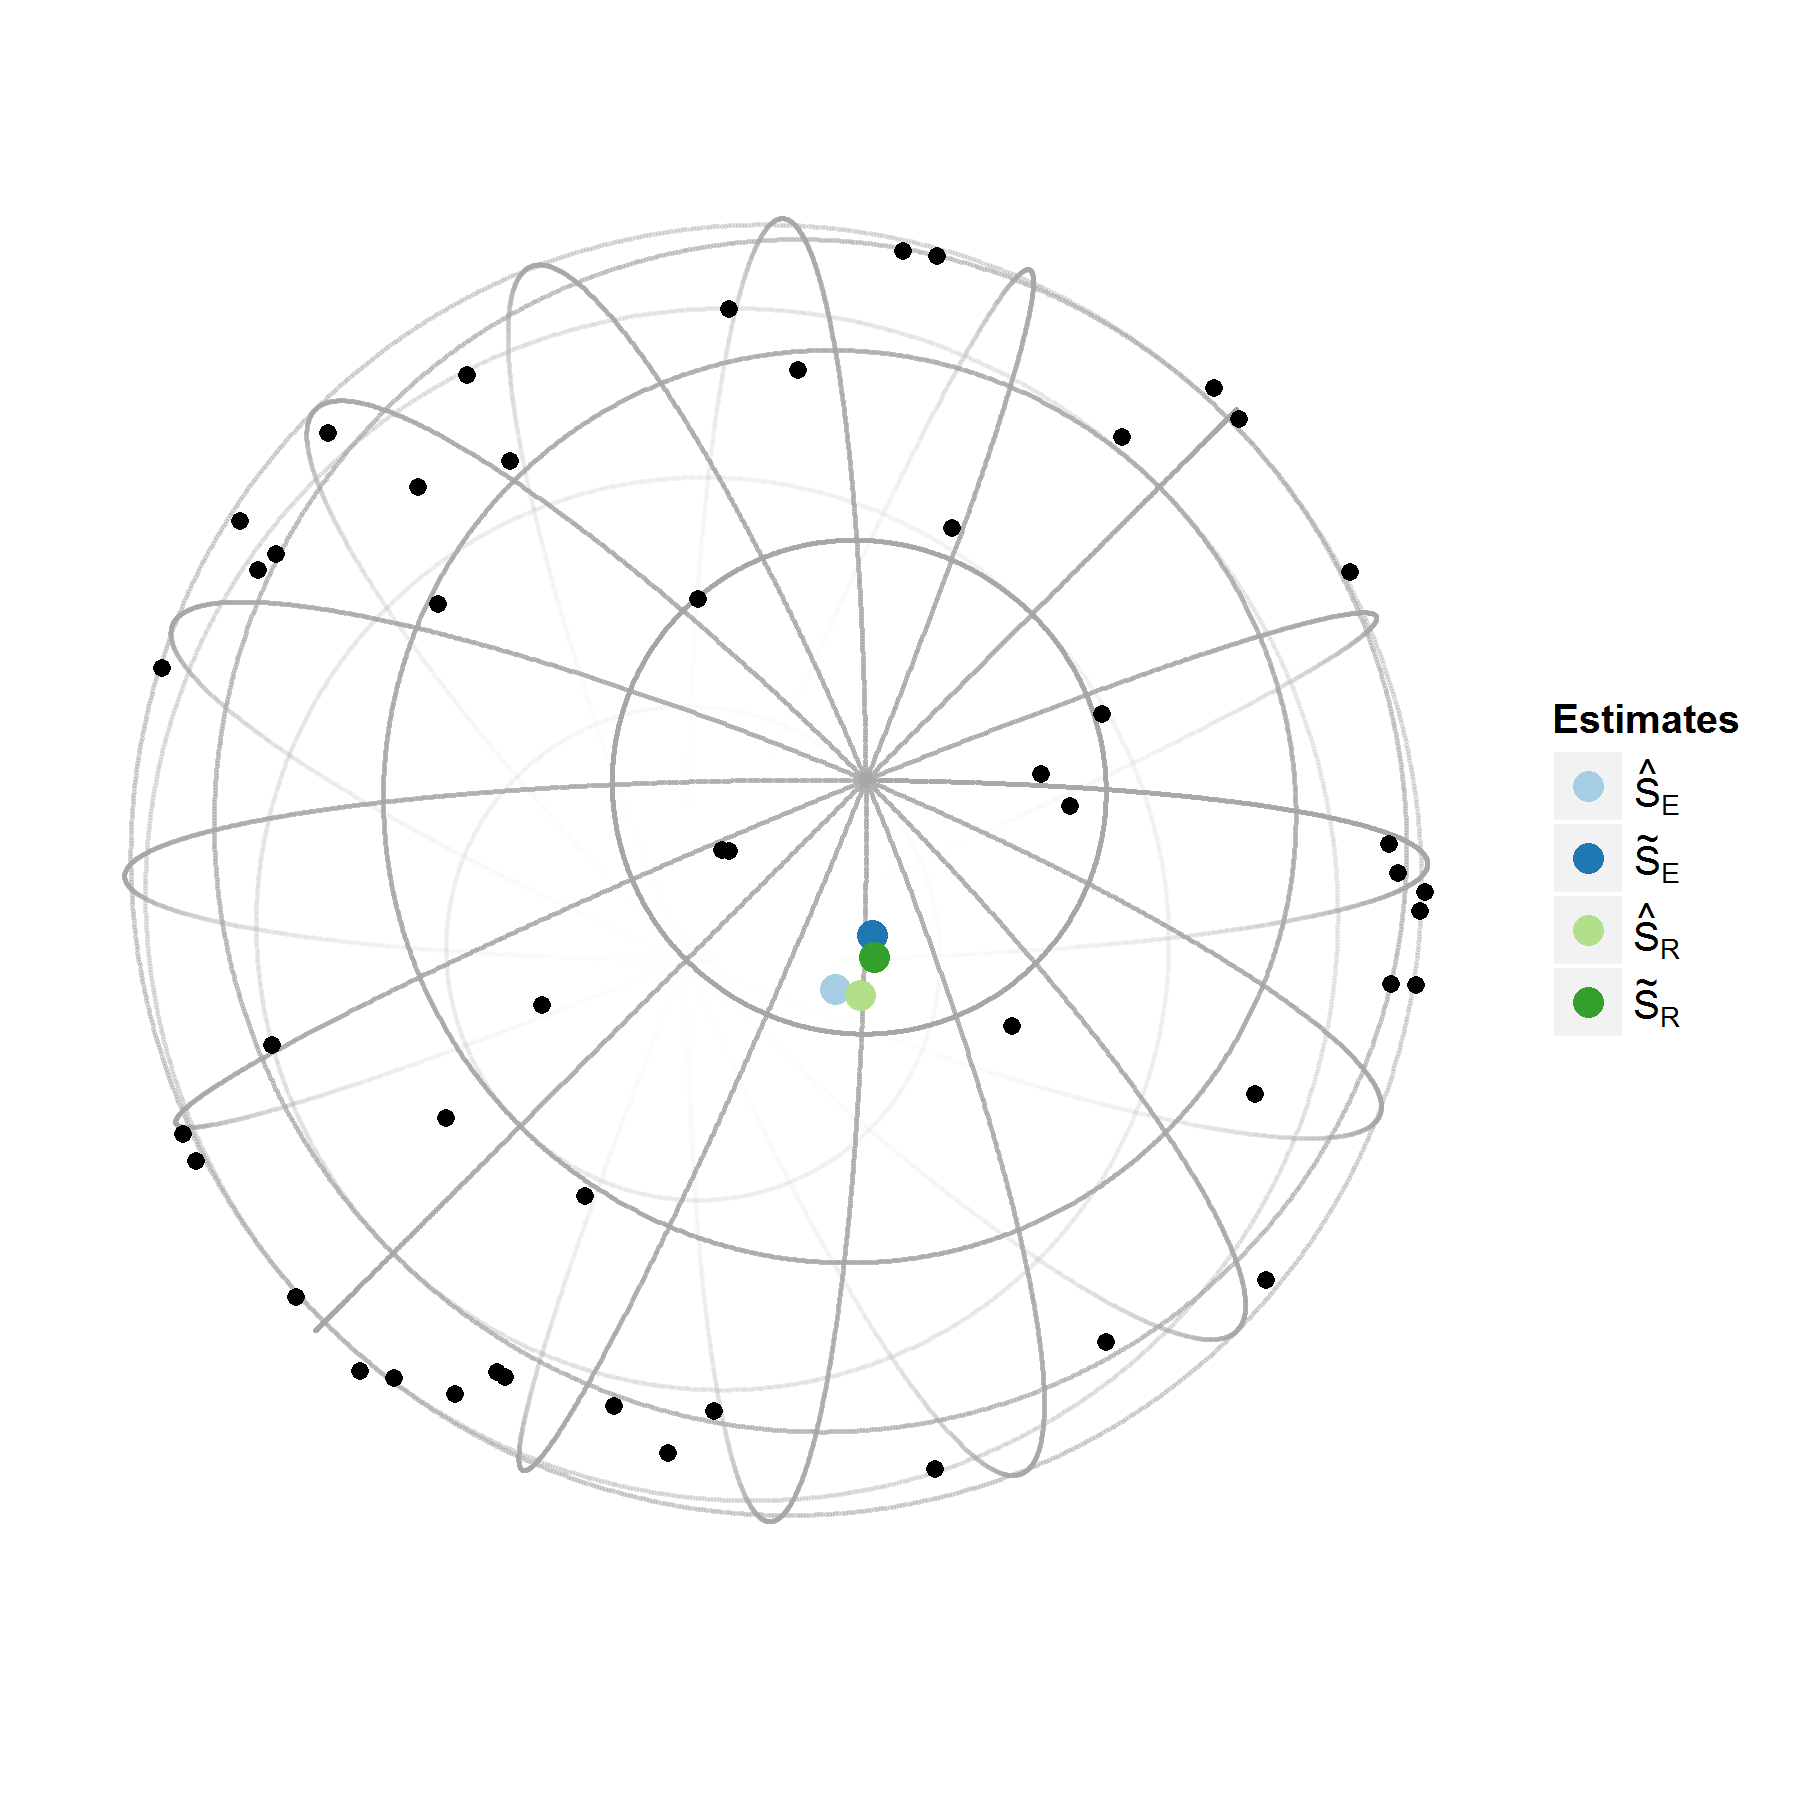
\includegraphics[width=.75\textwidth]{figures/eye2}
%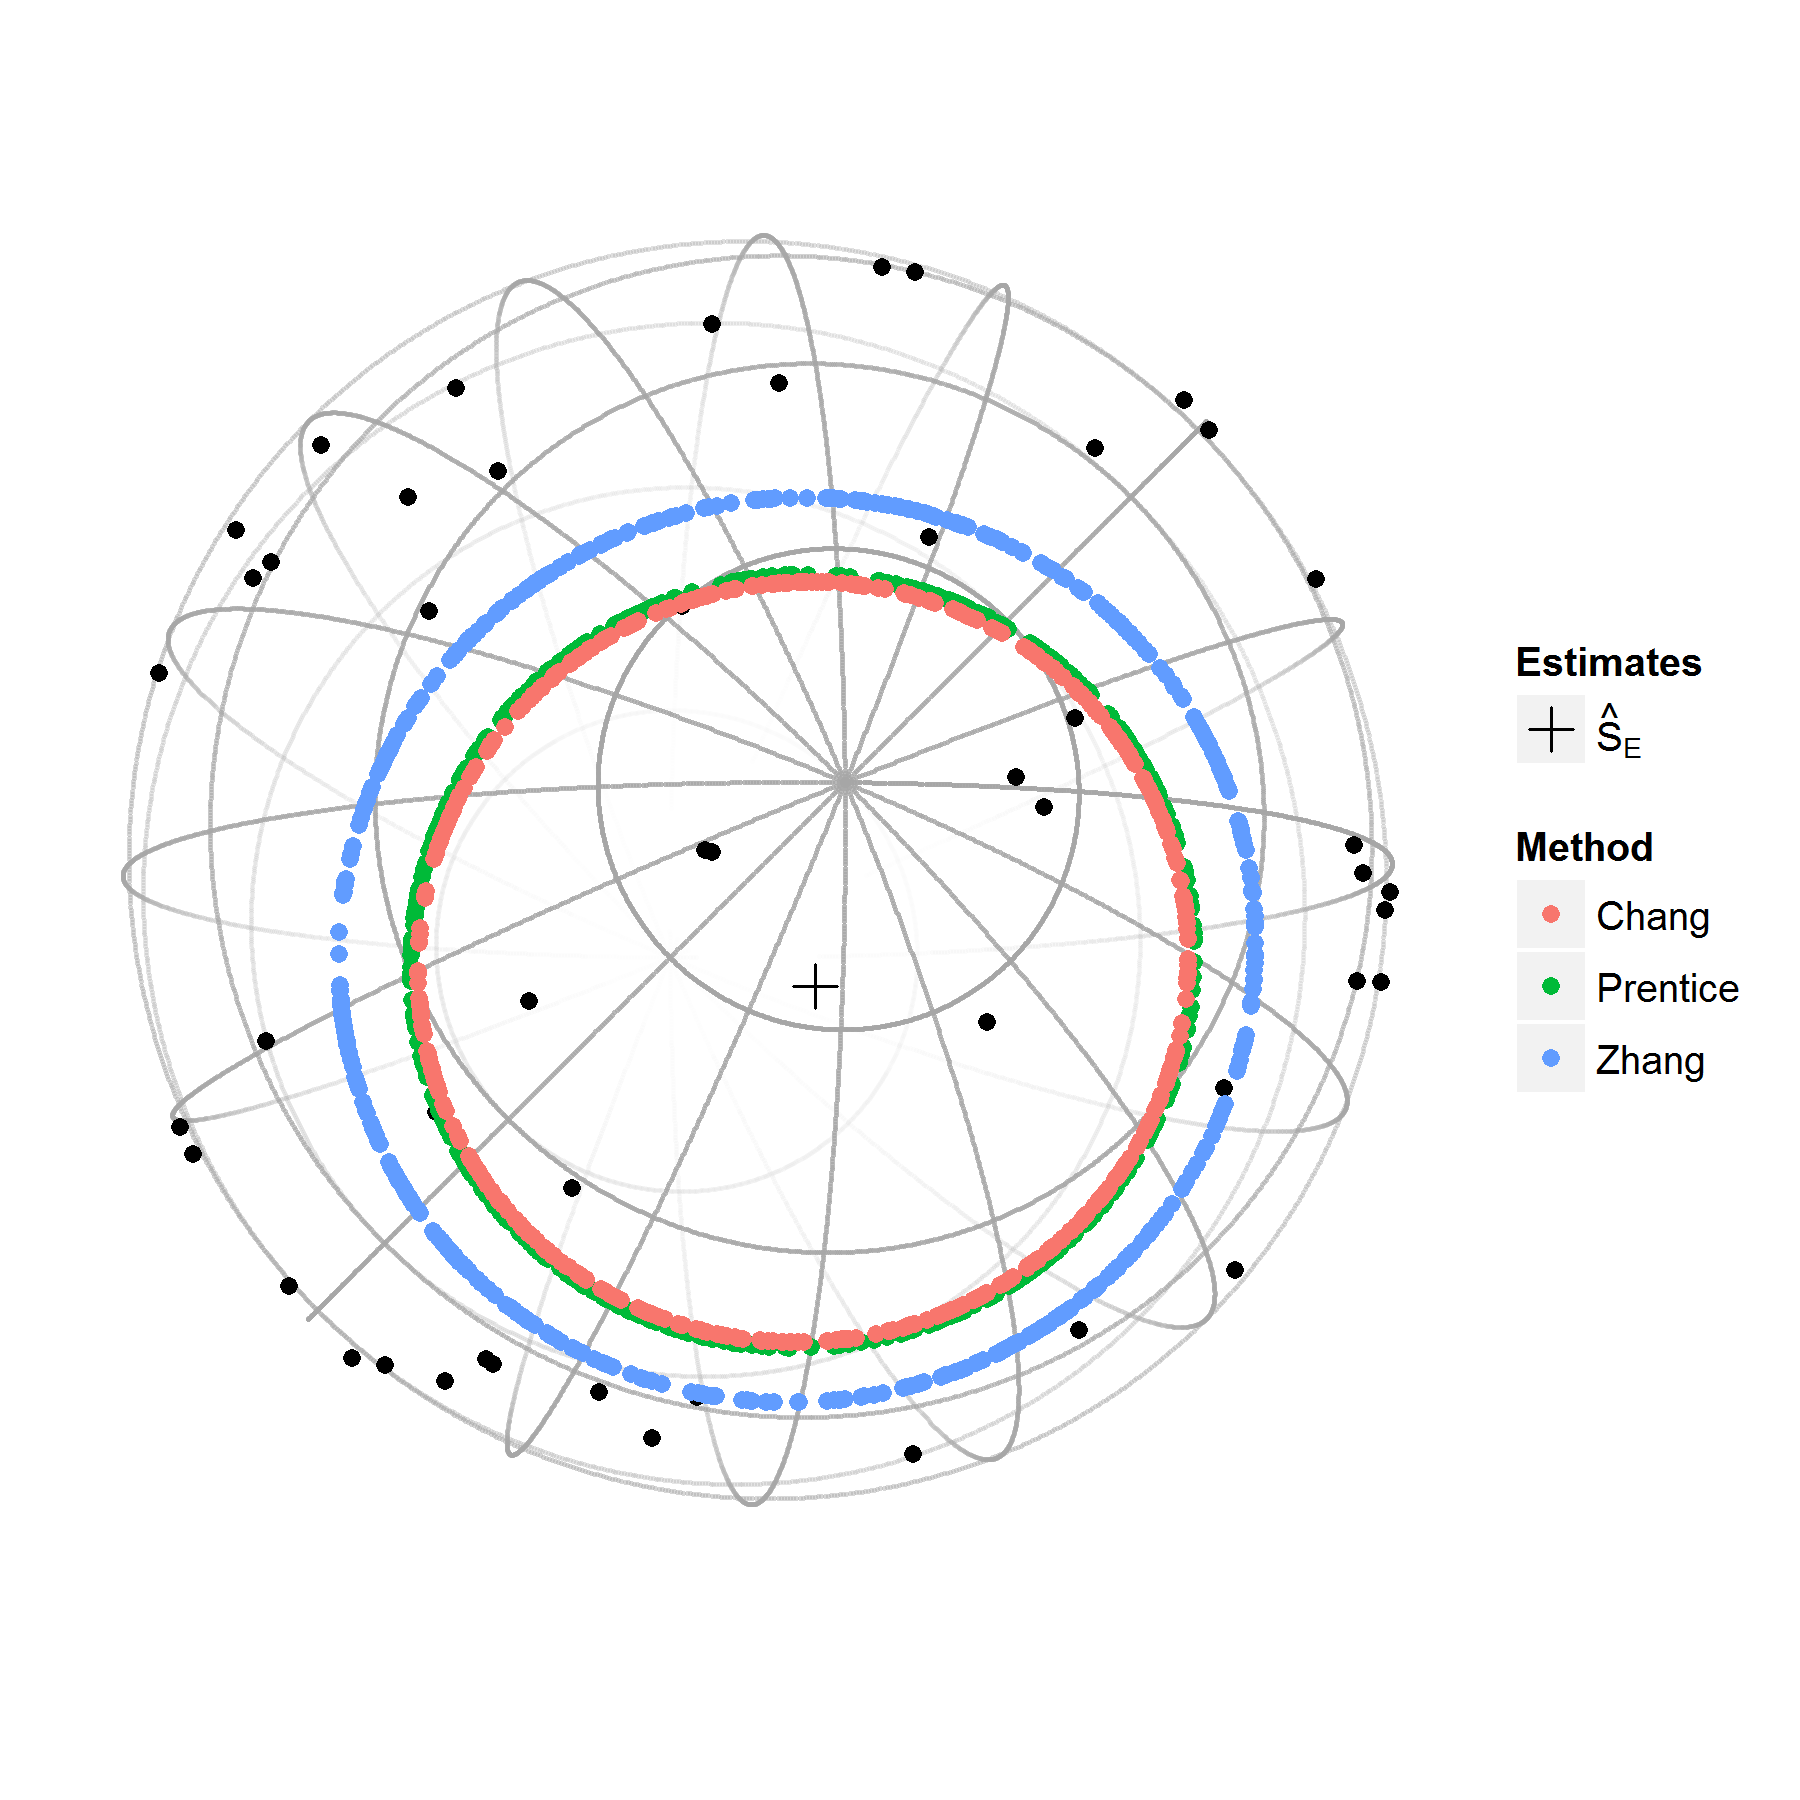
\includegraphics[width=.75\textwidth]{figures/eye3}
\caption{\label{figure:eye1}
A plot of the a random sample from the Cayley-UARS distribution with $\kappa=1$.}
\end{figure}

In Figure \ref{figure:eye1} a random sample of 50 matrices following the Cayley-UARS distribution with $\kappa=1$ is plotted along with four estimates of the central orientation.  The code to produce this plot is also given.

\section{Summary}

The \pkg{rotations} package is introduced and allows the user to create, simulate, analyze and visualize rotation data.  There are three parameterizations possible in this package and four built-in distributions from which data can be simulated.  The four estimators discussed in Stanfill et al. (2012) are each implemented and each can be visualized via \code{ggplot2}.

%\bibliography{../REFERENCES}
\bibliography{stanfill-hofmann-genschel}

\address{Bryan Stanfill\\
  Department of Statistics\\
  Iowa State University\\
  Ames, IA 50011}\\
\email{stanfill@iastate.edu}

\address{Heike Hofmann\\
  Department of Statistics\\
  Iowa State University\\
  Ames, IA 50011}\\
\email{hofmann@mail.iastate.edu}

\address{Ulrike Genschel\\
  Department of Statistics\\
  Iowa State University\\
  Ames, IA 50011}\\
\email{ulrike@mail.iastate.edu}